\chapter{Climate Records in SE Asia: Singapore versus Thailand}
\chapterauthor{Mudit Murarka and Bebe Phornprapha}

\maketitle

\section{Introduction}

\begin{figure}
  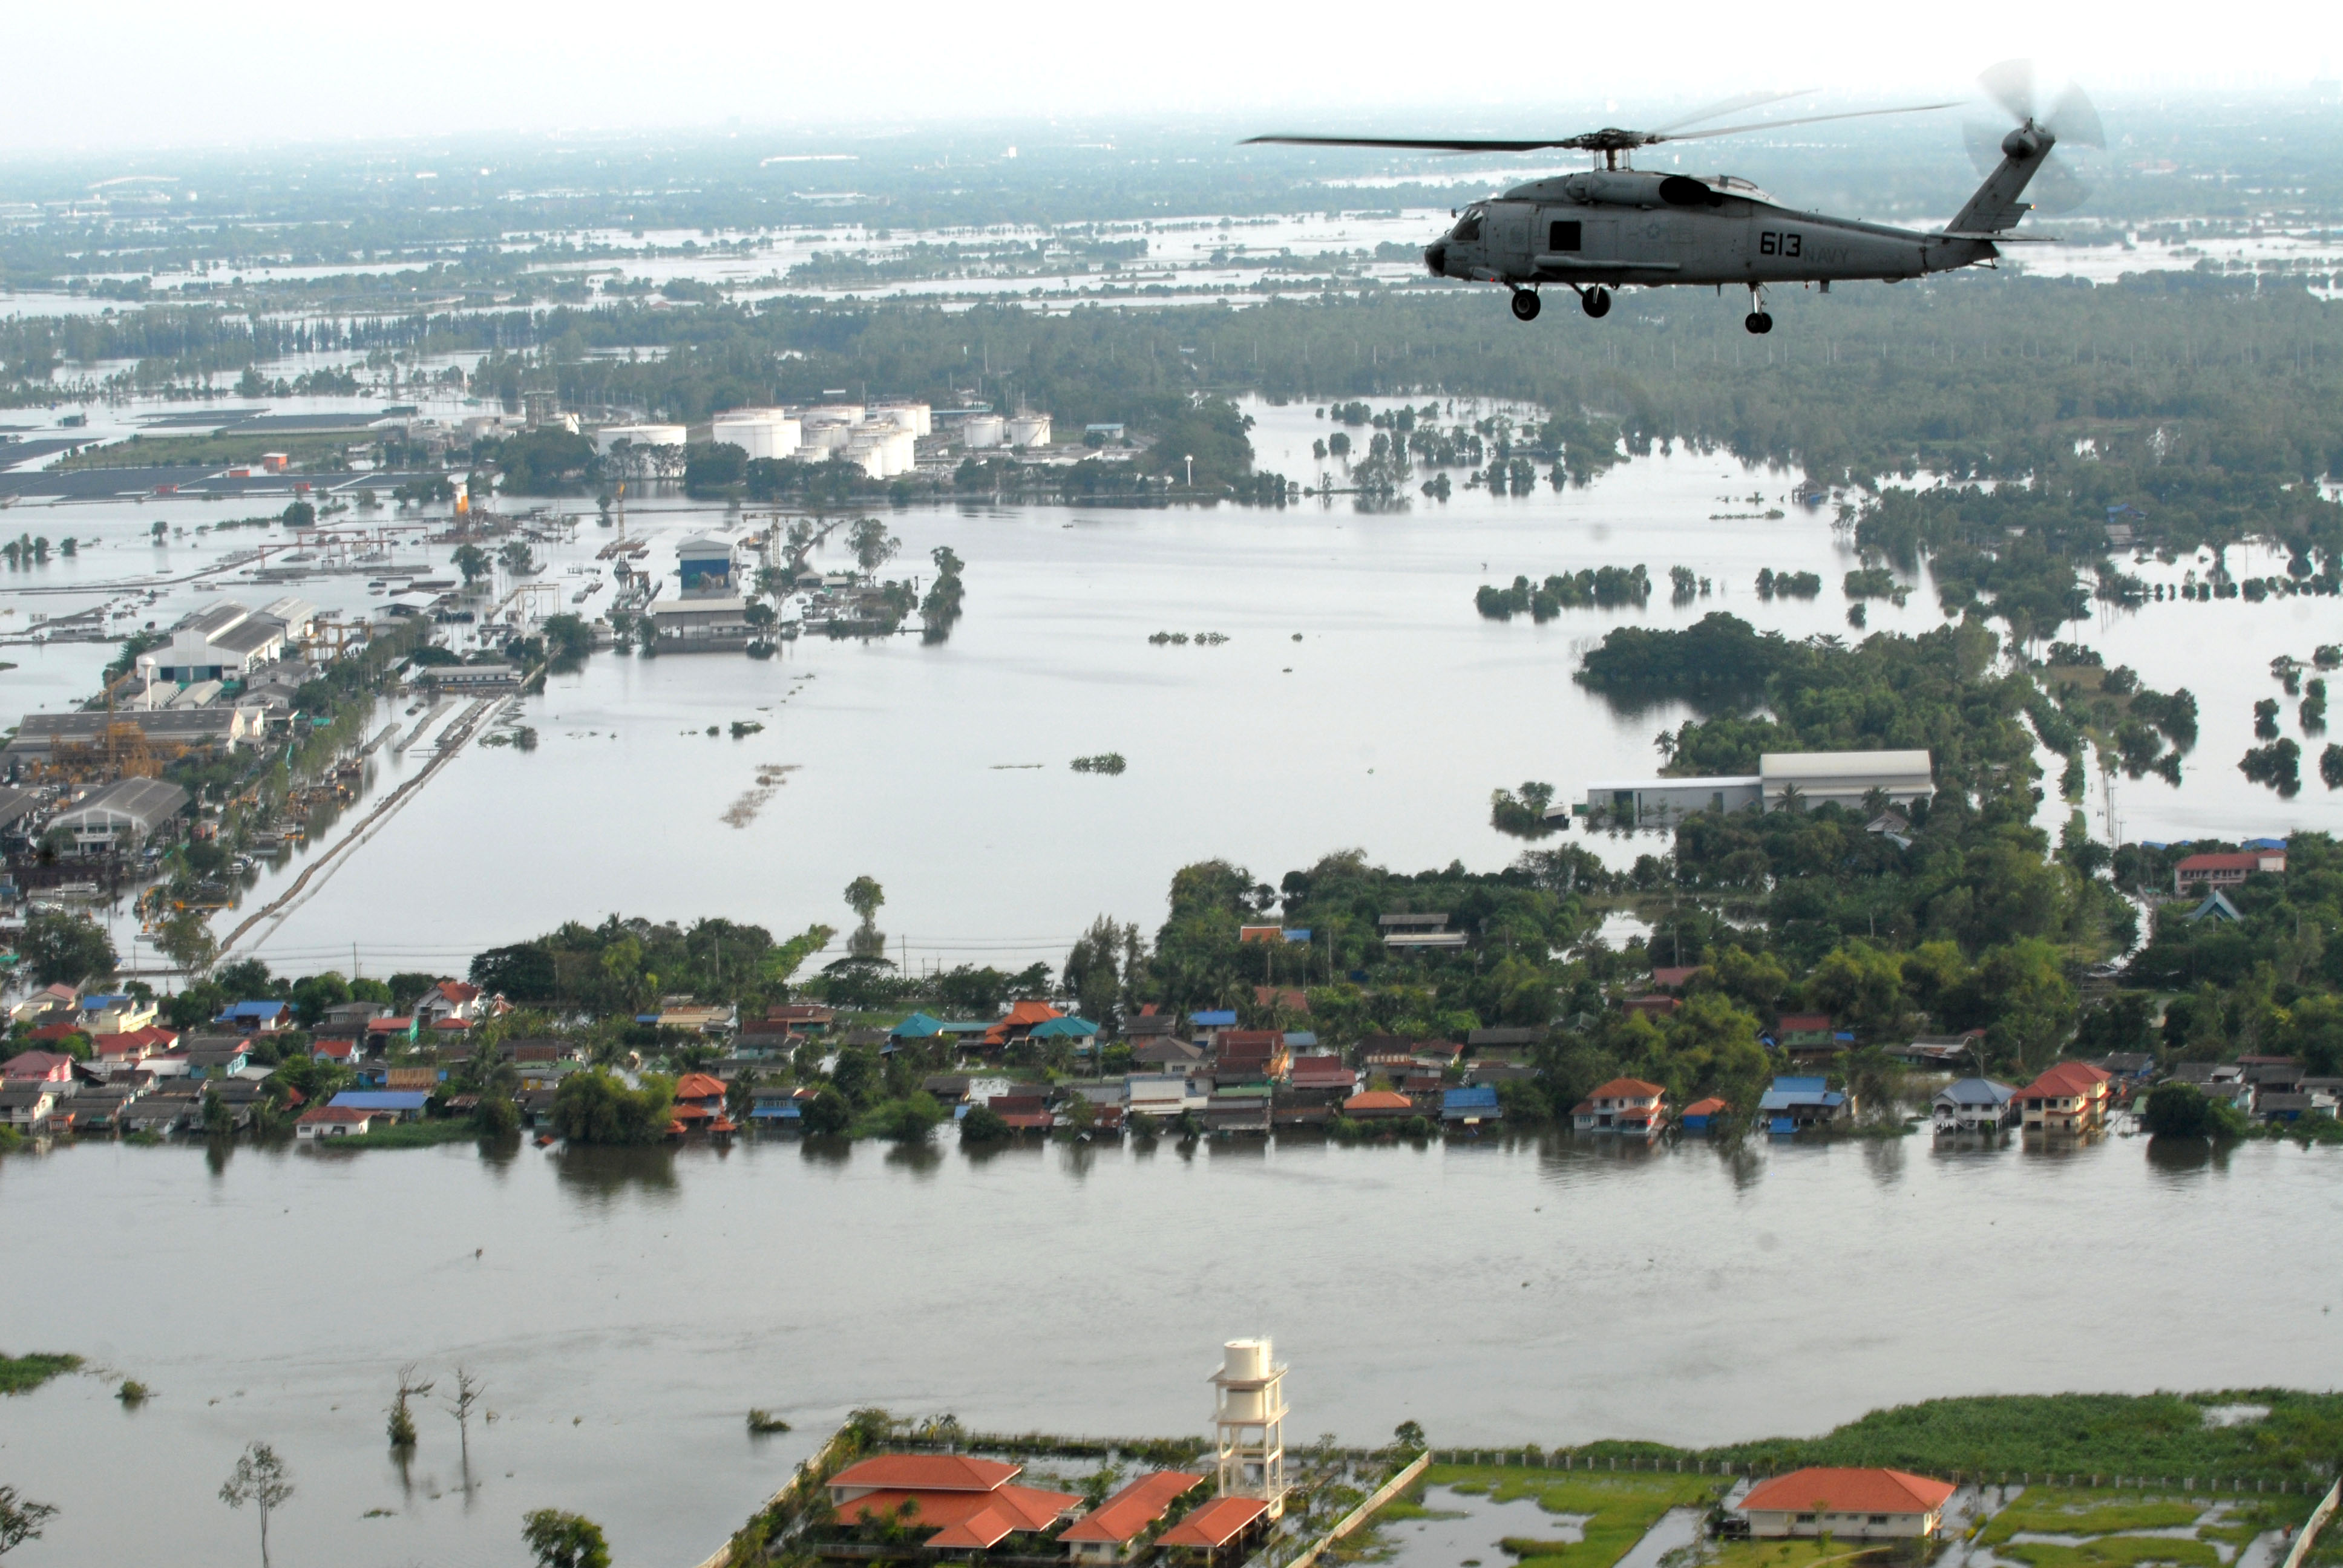
\includegraphics[width=\linewidth]{2011Floods}
  \caption{A US Navy helicopter observes the impact of the 2011 floods in the Bangkok area}
  \label{fig:2011floods}
\end{figure}

In 2011, Thailand was hit by its deadliest floods in over 50 years. 815 people were killed, and the Thai economy lost over over USD 30 billion. These floods occurred as a result of record rainfall over northern and central Thailand in early 2011. At the time, the Thai government may have thought of the flooding as a disaster which was to met by relief efforts in the short term  \citep{floodfailure}. However, it is now becoming clear that that the the flooding in 2011 may not have been an isolated incident.

Research suggests that the floods have a return period of about 10-20 years, i.e. a similar flood event is likely to occur within the next two decades\citep{galeandsaunders}. This occurence may have been acerbated by climate change; anthropogenic greenhouse gas emissions in Thailand have been tied to increase rainfall over the country, and, as these emissions increase, the potential for catastrophic flooding events will increase as well \citep{floodclimate}. 

The development of climate models such as the aformentioned one relating to the flood, and the monitoring of climatic variables is the function of the Thai Meteorological Department in Thailand. As in Thailand, meteorological agencies all over the world now have this function. Meteorology now has an essential role to play in the anticipation of and prepration for for the effects of future climate changes and natural disasters. Here, we will attempt to understand some of its foundations and illustrate its relevance. 


\subsection{What is meteorology and what are meteorological factors? What is their history?}

%- Aristotle is often called the father of meteorology. He wrote a volume titled Meteorology in 350 BCE that examined, among other things, the atmosphere, geology, geography and hydrology. \citet{aristotle} 

%- The history of weather observation networks operated by NOAA and its predecessor organizations in the United States goes all the way back to 1644. \citet{noaahistory}

%- \citet{meteopastpresent} provides a detailed history of the discipline of meteorology, all the way from the ancient period (Babylon, Ancient China, Aristotle, Theophrastus� Book of Signs) to the technological innovations that define the field today. 

%- \citet{mesoscale} provides an examination of the lack of spatiotemporally dense meteorological observations in Southeast Asia. The interior of Thailand is the only exception, due to a high concentration of observatories there. This study is a little outdated, but it�s the only one we could find analyzing the state of weather observation networks in Southeast Asia. 

%- \citet{meteonumbers} provides an examination of how meteorology became a discipline rooted in mathematics and physics following the Second World War, rather than a guessing game, as it was before. 

Meteorology can be defined as the field of study relating to the atmosphere, atmospheric phenomenon, and the effects of the atmosphere on our weather \citep{natgeodef}. It is an ancient field of study, dating back to at least the time of the Greeks. Aristotle is often called the father of meteorology. He wrote a volume titled Meteorology in 350 BCE that examined, among other things, the atmosphere, geology, geography and hydrology \citep{aristotle}. His successor,Theophrastus, also produced important work on meteorology, and contemporary ancient civilizations in Babylon and China also had an awareness of the discipline \citep{meteopastpresent}. 

Technological innovations have brought the discipline a long way since then. The discipline was especially transformed in the aftermath of of the Second World War, when it became rooted in mathematics and physics, rather than the more qualitative field it was before \citep{meteonumbers}. Today, most of the world depends on weather observation networks consisting of a combination of ground observers, who function largely as they did in ancient times, along with weather stations, satellites, radar, balloon borne sounding equipment and numerical weather prediction models \citep{britannicaforecasting}. These networks produce daily weather forecasts, which are a staple of modern life. 

In the United States, the history of weather observation networks operated by National Oceanic and Atmospheric Administration (NOAA) and its predecessor organizations  goes all the way back to 1644 \citep{noaahistory}. However, not all weather observation networks are as effective as NOAA's. For instance, there is a lack of spatiotemporally dense meteorological observations in Southeast Asia, outside of the interior of Thailand \citep{mesoscale}. 


\subsection{The relationship between weather and climate}

According to the National Snow and Ice Data Center in the United States, the definition of weather is the day-to-day state of the atmosphere, and its short-term variation in minutes to weeks. The definition of climate is the weather of a place averaged over a period of time, often 30 years. So, by continuously monitoring the weather, we can receive an indication of the state of our climate. Conversely, climate can tell us about statistical weather information, which can in turn tell us about the average weather, along with the range of weather extremes, for a location. By analyzing climate, we can then understand long term climate changes. This will help us figure out how to protect people from climate change \citep{climatevsweather}. 

Additionally, to predict the weather in the future, weather models can be used. Models take observations from weather observation networks and incorporate observations such as air pressure, temperature, humidity, and winds to produce the best estimate of current and future conditions in the atmosphere. So, models output the most likely scenario, which gives us short term weather forecasts, which can last up to a week. For long term weather forecasts, statistical relationships between large scale climate signals and precipitation and temperature generate predictions of what the weather will be like in one month to six months. Climate predictions can be made by using global climate models. However, climate models cannot use observations, as there are no observations from the future yet; thus climate models tend to be less reliable than weather models. \citep{nasaclimaterecords} 

\subsection{Why should we care about meteorology?}
As in the case of flooding in Thailand, good meteorlogical data has the potential to save lives. Since 1980, the number of natural disasters in the world and the number of people affected has risen. However, thanks to effective forecasting, the number of people killed has not risen. Today, an increasing number of people are situated in regions of high risk for weather hazards. Developing countries are going to be exposed to more extreme weather events due to climate change. The world�s population is exploding, city populations are exploding and weather/climate related diseases are now killing a million people every year. Most of the people are killed are children under the age of 5 in developing countries. Weather and climate forecasting is essential to combat all these problems \citep{preparedness}.For instance, weather forecasting was used to predict Typhoon Bopha in the Philippines in 2012, which helped mitigate a climate disaster. Through forecasting, Filipino citizens had information to wind speed, location of incoming weather disturbances, and possible amounts of precipitation. By predicting the Typhoon, the early warning Typhoon systems helped evacuate 167,000 people to shelters. Forecasting will continue to be incredibly important for this region in the future, as the IPCC predicts that that climate change is likely to cause tropical cyclones to become more severe with greater wind speeds and more intense precipitation.\citep{typhoon} 

In addition to the fact that effective meteorological systems can help save lives through effective hazard forecasting, they also have considerable economic benefits. These benefits result from the improved economic decisions that stakeholders can make with the knowledge that comes from meteorology. For instance, sound climatological meteorological information can help farmers make decisions about what crops to grow and when to grow them. It can help the energy industry in optimizing the generation, transmission and distribution of power. All in all, hydrometeorological information has significant impacts in the management of road traffic, railway traffic, the maritime industry, aviation, construction, energy, air quality and agriculture. A Swiss study found that that the cost-to-benefit ratio of meteorological services is likely between 1:4 and 1:6 \citep{swissmeteo}. A Chinese study found that the value of the benefit of the Chinese Public Weather Service was at least 46 billion Chinese Yuan in 2006 \citep{chineseservice}.  

\subsection{Analysis of Climate Records}
According to the IPCC, mean annual temperature is likely to have increased over the past century over most of the Asian region. Furthermore, it is likely that the numbers of cold days and nights have decreased and the numbers of warm days and nights have increased across most of Asia since about 1950 \citep{ipcc}.For this section, we will be analyzing trends in increasing rainfall and temperature in two countries in Asia: Thailand and Singapore. This was achieved by downloading the climate data from NOAA, and using the data to evaluate to evaluate long term climate patterns for these two countries. 

Singapore is affected by increasing temperatures, as from 1972 to 2014, the annual mean temperature has increased from 26.6�C to 27.7�C. As Singapore is an island, data was downloaded from the only weather station with data on temperature and precipitation.\citep{singaporeclimatechange}

Thailand is also affected by rising temperatures, and Average annualtemperatures have significantly risen by about 0.95� C between 1955 and 2009. Thailand has 53 weather stations, and so five stations were picked in different areas of the country for an overall climate assessment of the country. For  both Thailand and Singapore, data was first collected from 1950 until the present day. 

\subsubsection{Why were Singapore and Thailand chosen?}
Singapore and Thailand were chosen because both countries differ geographically and economically, yet are in close proximity to each other. Thailand is much larger than Singapore, and has a size of 513,120 km�, compared to Singapore�s 719.9 km�. Due to Thailand�s large size, it is split up into 76 provinces, with most of the development and economic resources concentrated in the capital, Bangkok. However, Singapore is a island, and so the development and economic resources are mostly tantamount for the entire country. Both countries are found near the equator and are 945 km away from each other, and so the climate for Singapore and Thailand, especially Southern Thailand, should be similar to each other. By analyzing these two countries, climate and rainfall can be compared between a small developed and a large developing country.

\subsubsection{Which areas were chosen within each country?}

As Singapore is a small island with one weather station, that station was chosen. 

However, five geographically different locations with different degrees of development in Thailand were chosen in order to get an accurate representation of weather in the country. Bangkok (a urban area in the center), Chiang Rai (a urban-rural area in the North West), Sakon Nakhon (a rural area in the North East), Phuket (a urban area in the South West), and Nakon Si Thammarat (a urban-rural area in the South East) were chosen. These stations are illustrated in Figure \ref{fig:stationsmap}

\subsubsection{What months were picked?}

For Singapore, January, May, and November were selected. These months were chosen because January is the coldest month, May is the hottest month, and November is the rainiest month \citep{singaporeweather}. 

For Thailand, January, April, August were selected. These months were chosen because January is the coldest month, April is the hottest month, and August is the rainiest month \citep{thailandweather}. 

\begin{figure}
  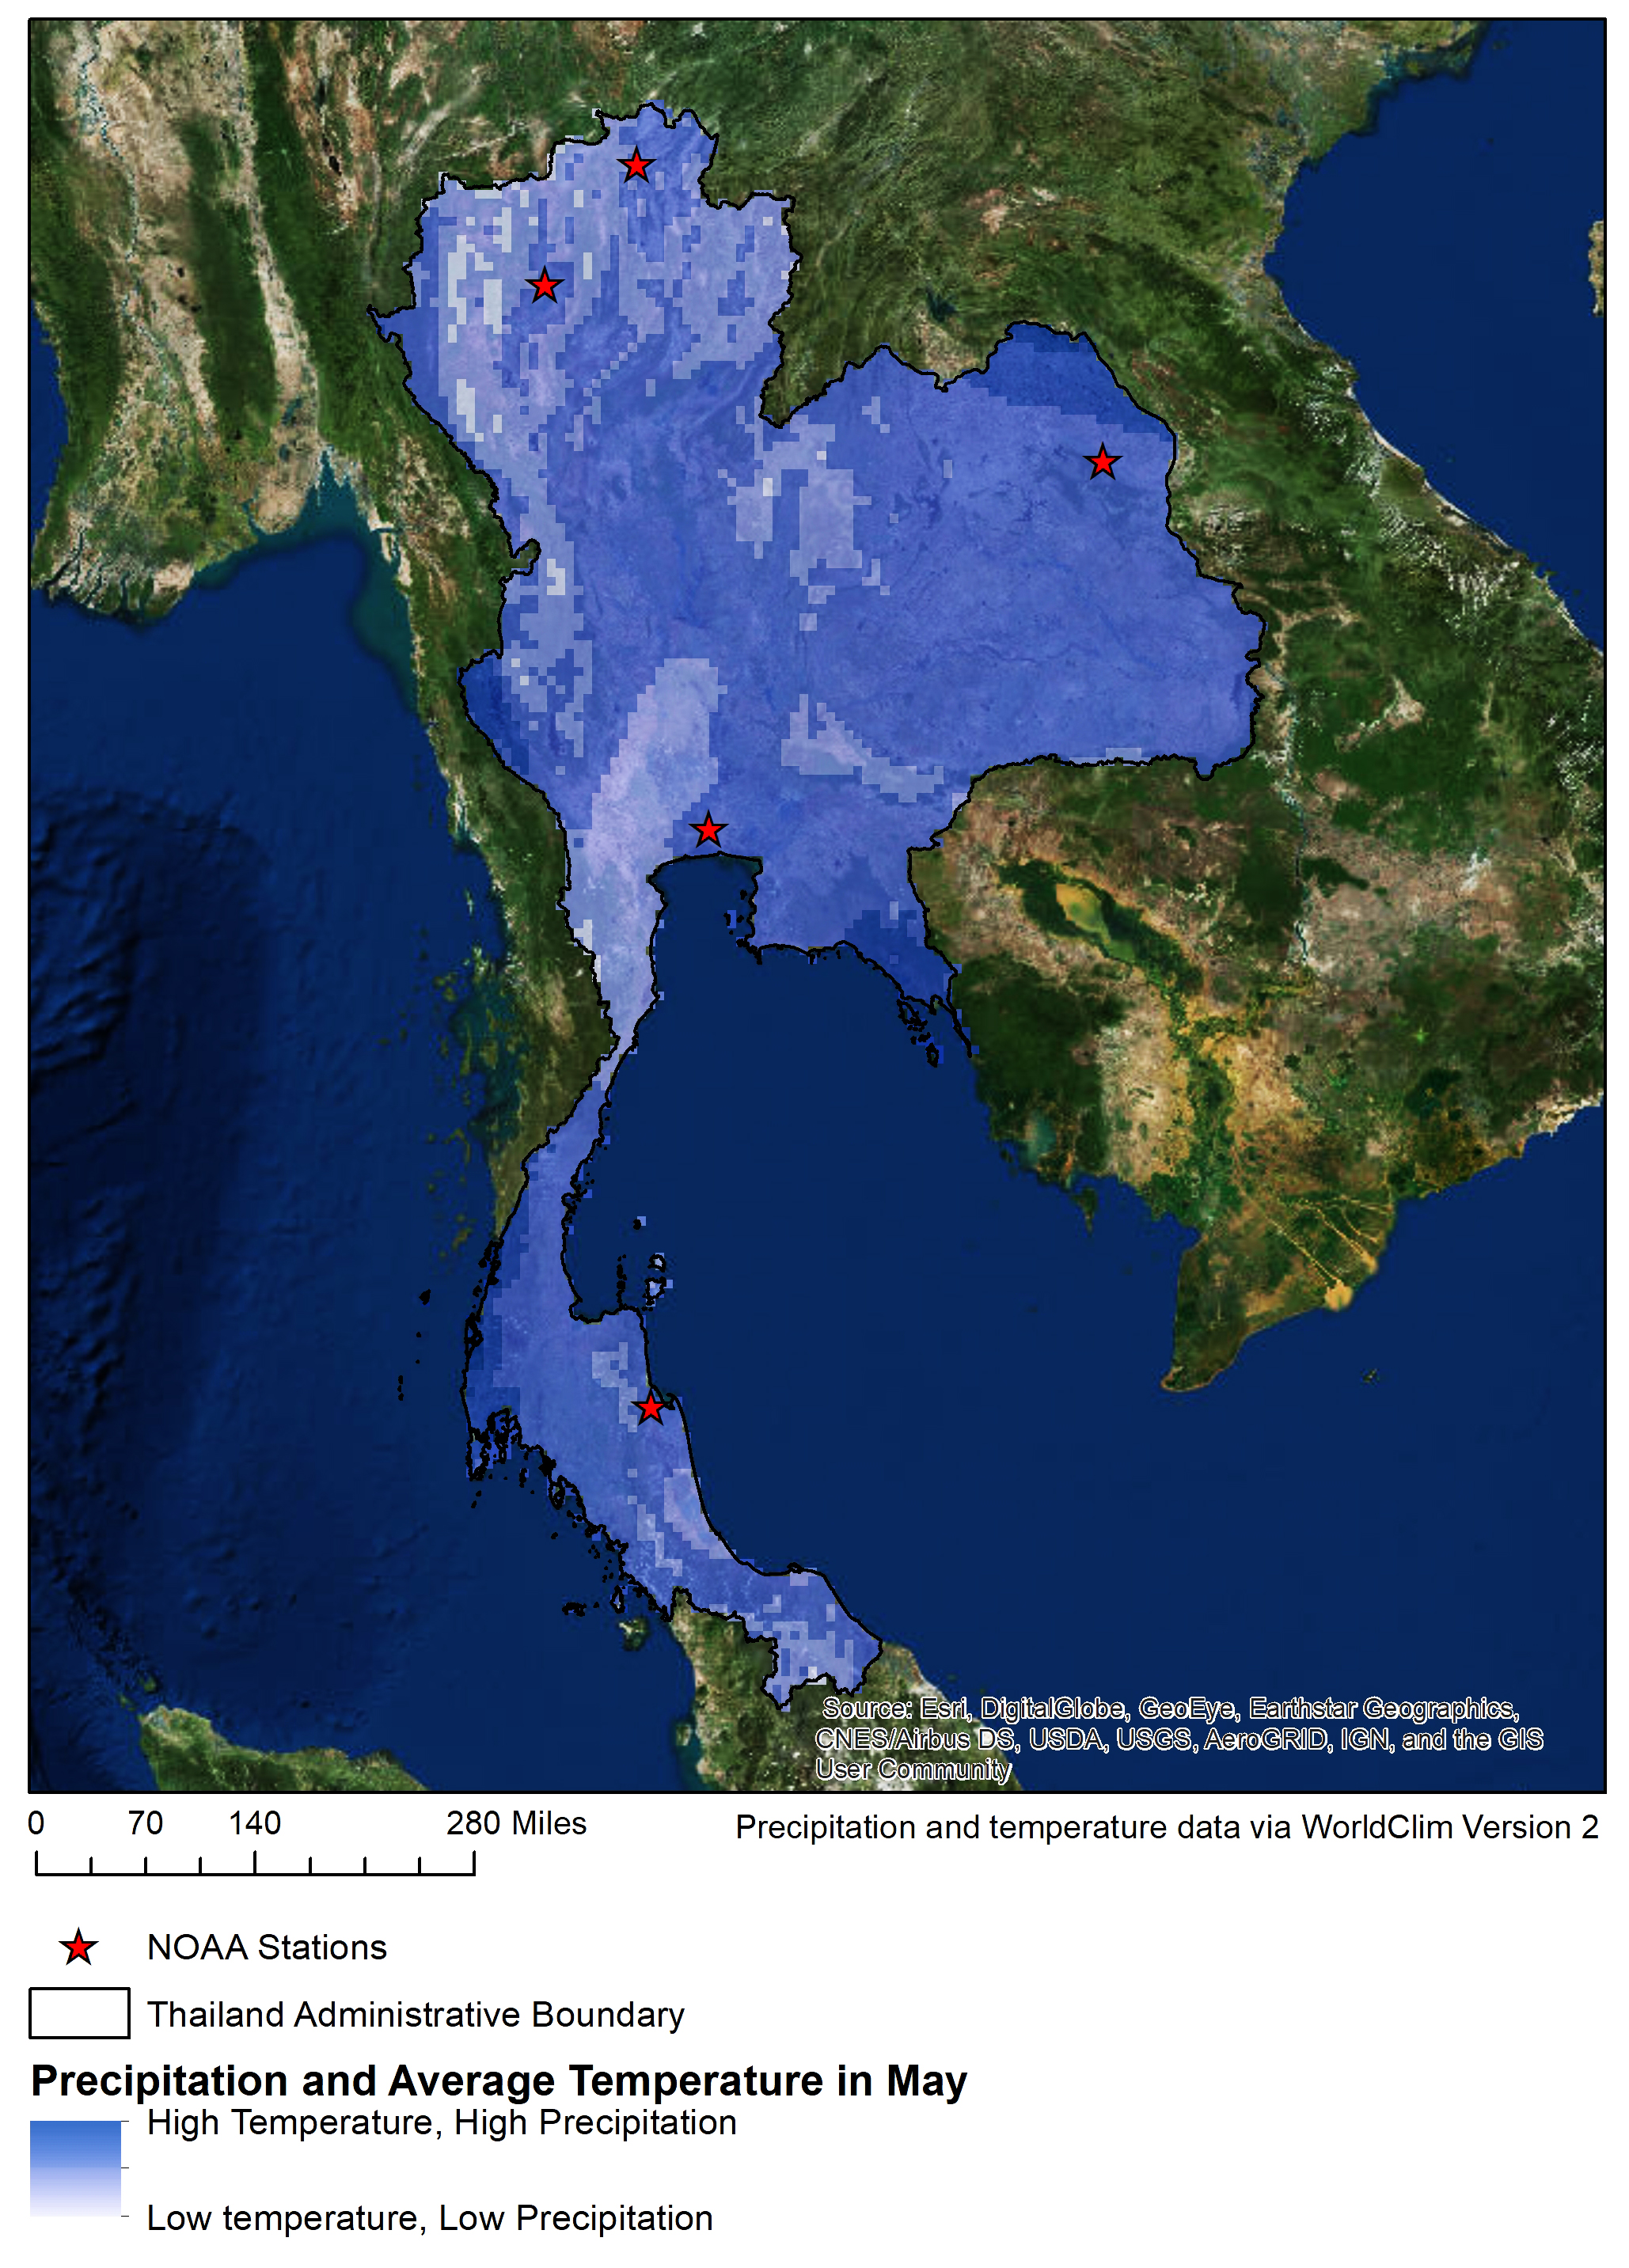
\includegraphics[width=\linewidth]{ClimateMapEnhanced}
  \caption{The NOAA stations in Thailand chosen for analysis in this chapter. They are depicted on top of a raster which shows the prevailing average temperatures and humidity in Thailand in May. This is to help indicate why these particular NOAA stations were chosen.}
  \label{fig:stationsmap}
\end{figure}

\section{Climate Data}

\subsection{What is graphed?}
A linear regression of Monthly Average Rainfall and Maximum Temperature are graphed below. Monthly Average Rainfall can analyze changes in precipitation, and Maximum Temperature can attest to change in temperature. Maximum temperature is chosen over average temprature because there is not a strong enough trend for average temperaure. Reasons for this are not apparent, and more reserach should be done on this subject.  

\subsection{Overall Temperature Trend}
From 1880, global surface temperature has increased 0.07�C every 10 years. However, the past century has seen a warming of 0.74�C. \citep{tempincrease}. Both Thailand and Singapore have seen an increase in maximum temperature.

\subsubsection{Singapore}
Major climate models show that Singapore has warmed gradually by about 0.25 deg C in each decade from 1948 to 2015, and that temperatures will continue to increase. In our temperature analysis, we found out that Singapore's maximum temperature has been increasing from 1950 to the present day for the months of May, November, and January. For all three months, there are positive upwards trend line and statistically significant results. The p-value for all three months is less than 0.05, and thus statistically significant. \citep{singaporeweather}

\begin{figure}[h!]
\centering
  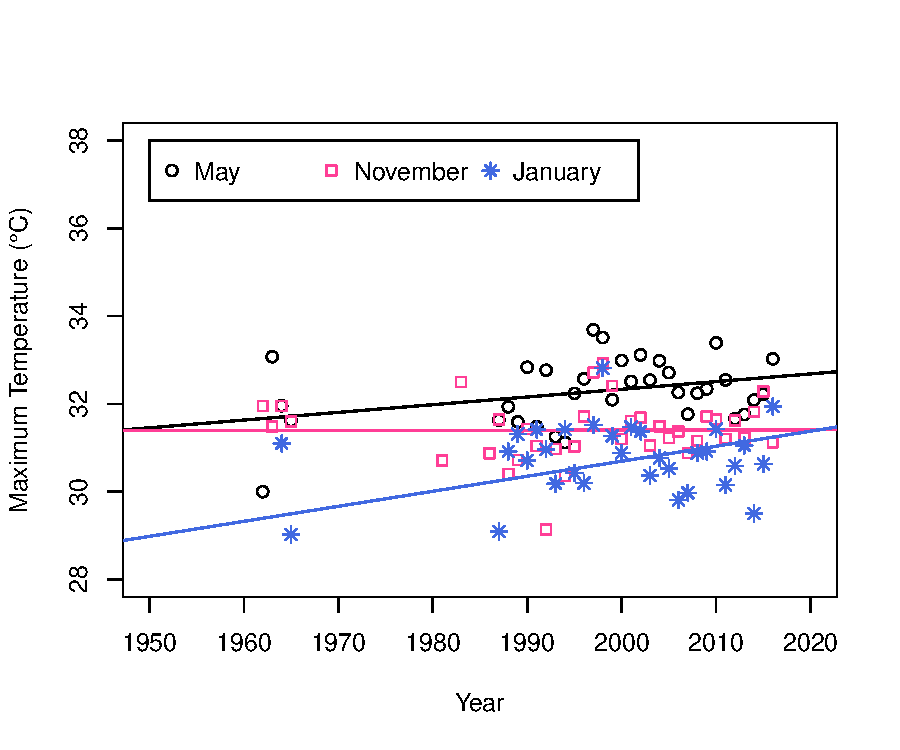
\includegraphics[width=.8\linewidth]{TMAX_Singapore}
  \caption{Average Monthly Maximum Temperature in Singapore}
  \label{fig:TMAX_Singapore}
\end{figure}

\subsubsection{Thailand}

Major climate models indicate a temperature rise for the whole country of Thailand, particularly the central plain and lower North-eastern region. However, there is no specific literature analysing the picked regions. Projections show that mean temperatures in central Thailand, including Bangkok, has been increasing by 0.4 in each decade from 1958 to 2014. In our temperature analysis, we found that Thailand's maximum temperature is increasing overall for all five locations, however, not every month is statistically significant. On the other hand, Bangkok seems to show a significant trend which is congruent with the predictions that central Thailand�s temperature will be increasing.  \citep{bkkweather}

\textbf{Bangkok}: Bangkok's maximum temperature has been increasing from 1950 to the present day for the months of April, August, and January. All three months have steep upward positive trend lines, and all three months are statistically significant, as the p value for all months is lower than 0.05.

\begin{figure}[h!]
  \centering
  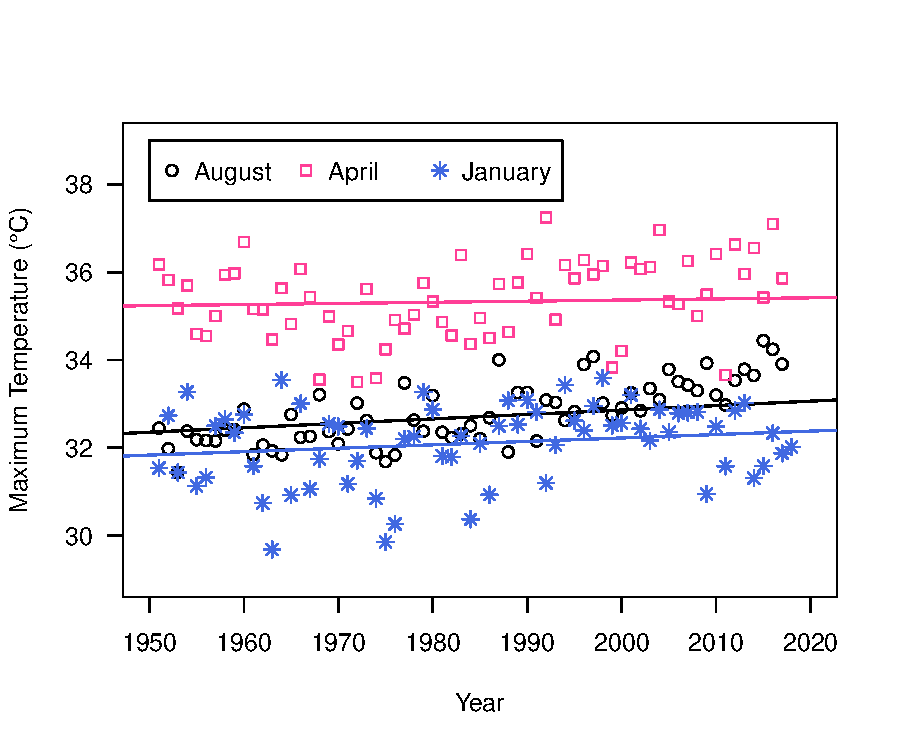
\includegraphics[width=.8\linewidth]{TMAX_Bangkok}
  \caption{Average Monthly Maximum Temperature in Bangkok}
  \label{fig:TMAX_bangkok}
\end{figure}

%\textbf{Chiang Rai}: Chiang Rai's maximum temperature has been increasing from 1950 to the present day for the months of August and January. Both of these months have steep upward positive trend lines, and are statistically significant, as the p value for both months is lower than 0.05. April has a downards gentle negative line trend, showing a decrease in maximum temperature. However, the p value is 0.326, larger than 0.05, and so this result is not statistically significant. 





%\textbf{Sakon Nakhon}: Sakon Nakhon's maximum temperatu%re has been increasing from 1950 to hte present day for %the month of August. There is a steep positive trend %line with a statistically significant p value lower %than 0.05. However, the months of January and April %have a horizontal trend line, with p values of 0.96 and 0.99, very statistically insignificant.

%\begin{figure}[h!]
%  \centering
%  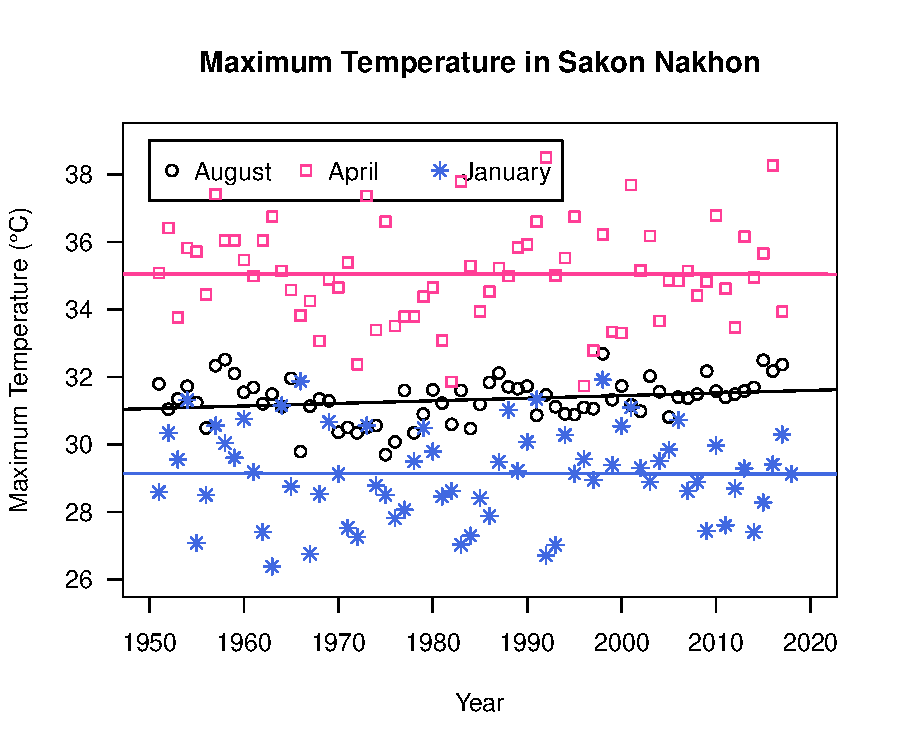
\includegraphics[width=.8\linewidth]{TMAX_Sakon}
%  \caption{?? in Sakon}
%  \label{fig:TMAX_Sakon}
%\end{figure}


%\textbf{Nakon Si Thammarat}:Nakon Si Thammarat's maximum temperature has been increasing from 1950 to the present day for the months of April, August, and January. January and August have steep upward positive trend lines, with statistically significant p values lower than 0.05. However, April, which has a positive upward trend line, has a pvalue of 0.127, which is statistically insignificant.  

%\begin{figure}[h!]
%  \centering
 % 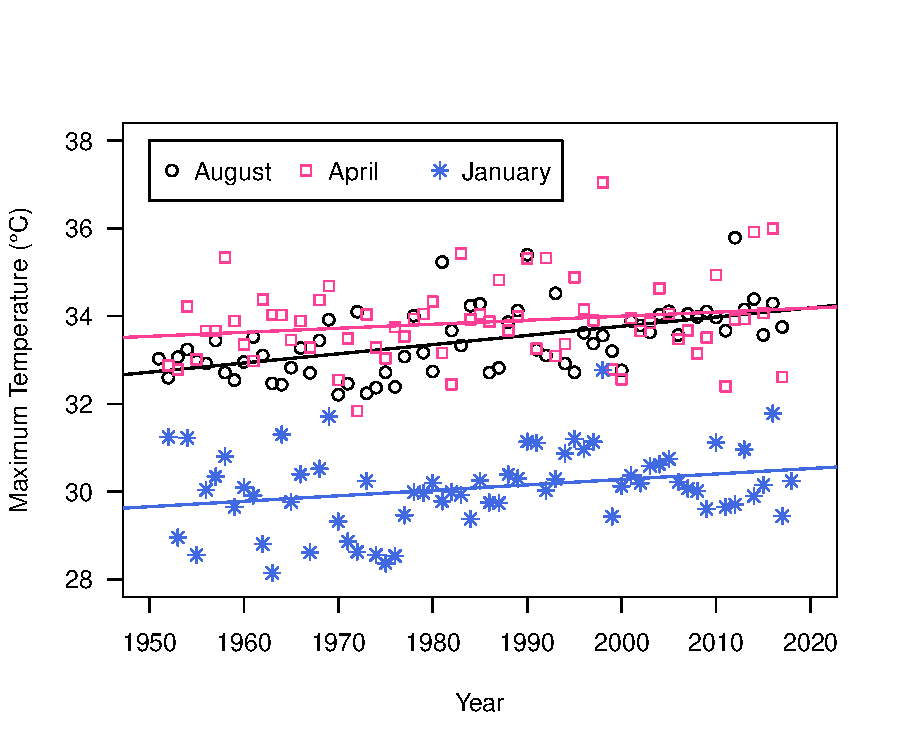
\includegraphics[width=.8\linewidth]{TMAX_Nakon}
%  \caption{?? in Nakon}
%  \label{fig:TMAX_Nakon}
%\end{figure}

%\textbf{Phuket}: Phuket's maximum temperature has been increasing from 1950 to the present day for the months of April, August, and January. All three months have steep upward positive trend lines, and all three months are statistically significant, as the p value for all months is lower than 0.05. 

%\begin{figure}[h!]
%\centering
%  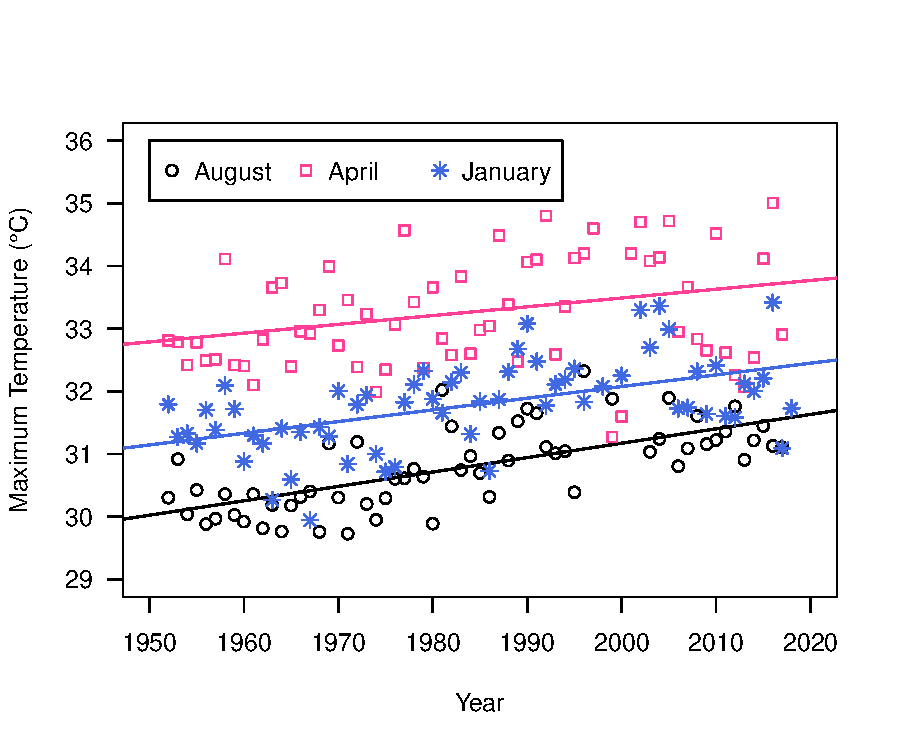
\includegraphics[width=.8\linewidth]{TMAX_Phuket}
 % \caption{?? in Phuket}
%  \label{fig:TMAX_Phuket}
%\end{figure}

\subsection{Overall Rainfall Trend}
According to the IPCC, the annual total wet-day rainfall in South East Asia has increased by 22 mm per decade, while rainfall from extreme rain days has increased by 10 mm per decade. Furthermore, between 1955 and 2005 the ratio of rainfall in the wet to the dry seasons increased, and there has been an increasing in frequency of extreme rainfall events in the northern parts of Southeast Asia. \citep{IPCC}

\subsubsection{Singapore}
Rainfall in Singapore has become more intense in recent years. According to Singapore's Second National Climate Change Study, there has been a general uptrend in annual average rainfall from 2192mm in 1980 to 2727mm in 2014 \citep{singaporeclimatechange}. In our rainfall analysis, we found out that  Singapore's monthly average rainfall has been increasing from 1950 to the present day for the months of May, November, and January. For all three months, there is a positive upwards trend line and statistically significant results. The p value for all three months is less than 0.05, and thus statistically significant.   

\begin{figure}[h!]
\centering
  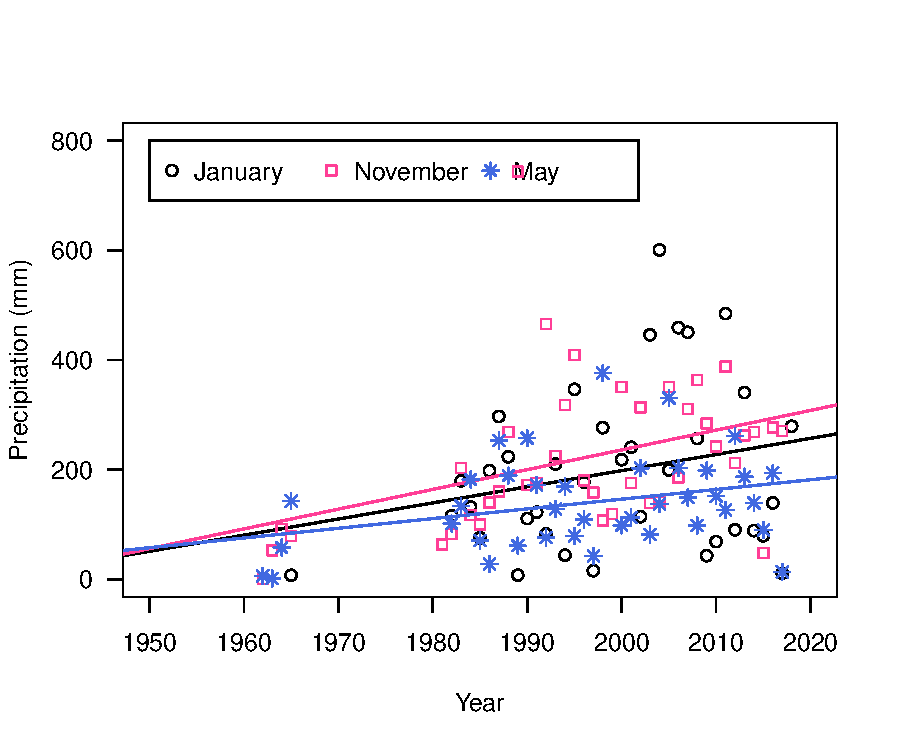
\includegraphics[width=.8\linewidth]{PRCP_Singapore}
  \caption{Monthly Average Rainfall in Singapore}
  \label{fig:PCRP_singapore}
\end{figure}


\subsubsection{Thailand} 
There has been no significant change of rainfall volume in Thailand, and the total amount of rainfall between 1955 and 2014 did not change significantly. However, there has been evidence that there has been increasing rainfall in the Northeast and Gulf region as well as the Bangkok area. \citep{bkkweather}. In our rainfall analysis, there is no clear trend for Thailand�s monthly average rainfall. For some areas, rainfall is increasing, and for some areas rainfall is decreasing. However, Bangkok's monthly average rainfall is increasing. 

\textbf{Bangkok}: Bangkok's monthly average rainfall has been increasing from 1950 to the present day for the months of August and January. Both these months have steep upward positive trend lines, and are statistically significant, as the p values are lower than 0.05. However, August which has a downward negative trend line, has a p value larger than 0.05, which is statistically insignificant. 

\begin{figure}[h!]
  \centering
  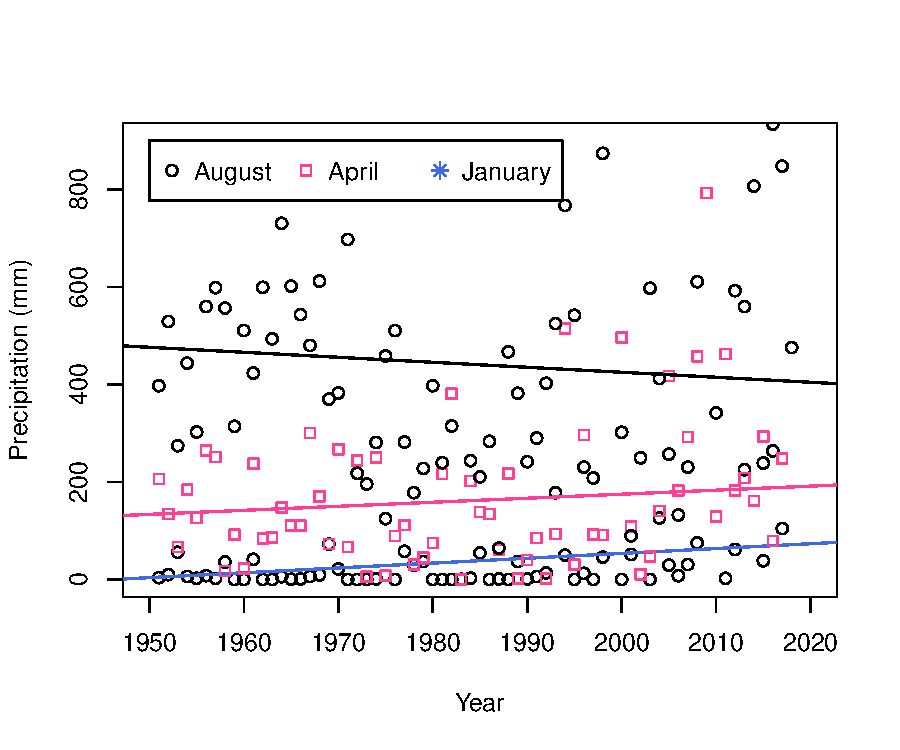
\includegraphics[width=.8\linewidth]{PRCP_Bangkok}
  \caption{Monthly Average rainfall in Bangkok}
  \label{fig:PRCP_bangkok}
\end{figure}

%\textbf{Chiang Rai}: Chiang Rai's monthly average rainfall has been increasing from 1950 to the present day for the months of April and January, but decreasing for August. However, the p values for all three months are larger than 0.05, proving the results to be statistically insignificant. 

%\begin{figure}[h!]
 % \centering
  %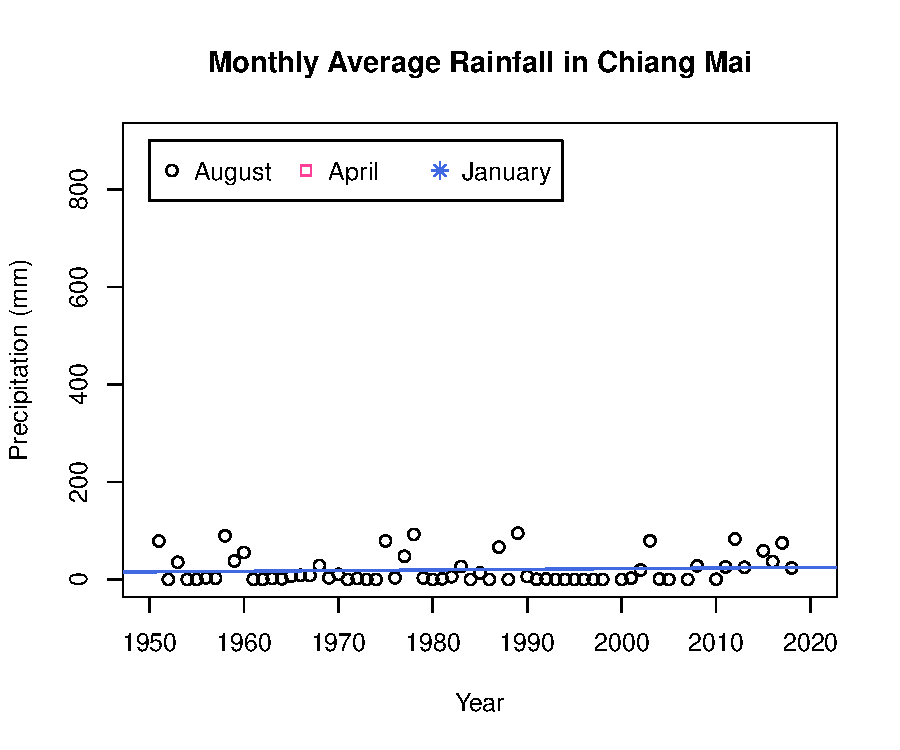
\includegraphics[width=.8\linewidth]{PRCP_Chaingrai}
 % \caption{?? in Chaingrai}
  %\label{fig:PCRP_chaingrai}
%\end{figure}

%\textbf{Sakon Nakhon}: Sakon Nakhon's monthly average rainfall has been increasing from 1950 to hte present day for the months of August, April, and January. While all three curves for slope upwards, the gradient is rather gentle. Furthermore, the p values for all three curves are larger than 0.05, deeming the results as insignificant.

%\begin{figure}[h!]
 %\centering
  %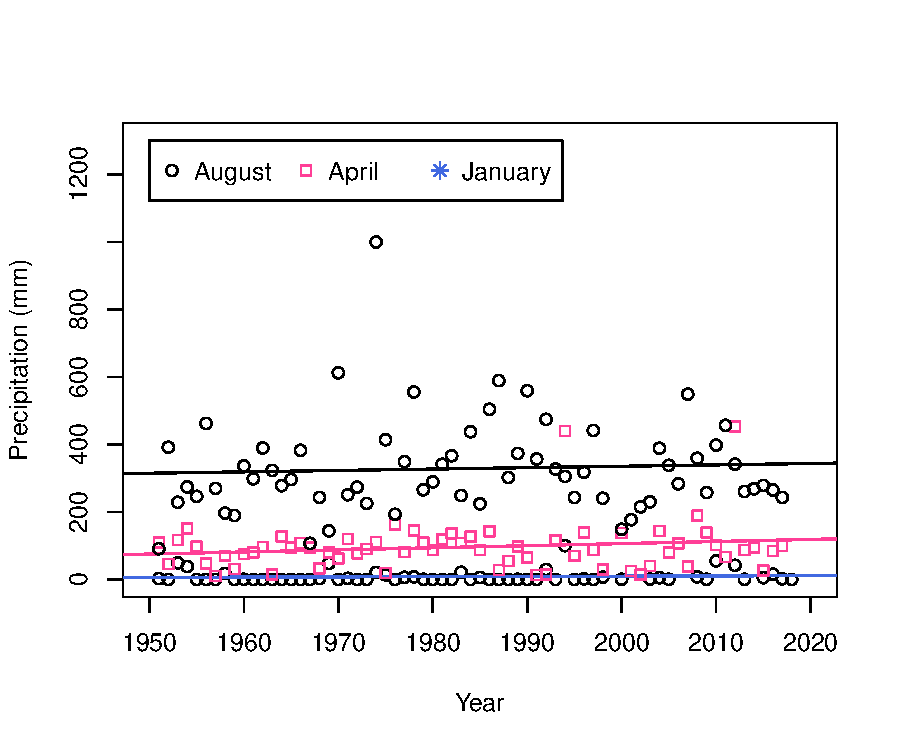
\includegraphics[width=0.8\linewidth]{PRCP_Sakon}
  %\caption{?? in Sakon}
  %\label{fig:PCRP_Sakon}
%\end{figure}

%\textbf{Nakon Si Thammarat}:Nakon Si Thammarat's monthly average rainfall has been increasing from 1950 to the present day for the months of April, August, and January. January has a steep postive upward trend line, and has a p value lower than 0.05, a statistically significant result. August and April both have an upward positive curve. However, the p values for both curves are larger than 0.05, a statistically insignificant result.  

%\begin{figure}[h!]
%\centering
 % 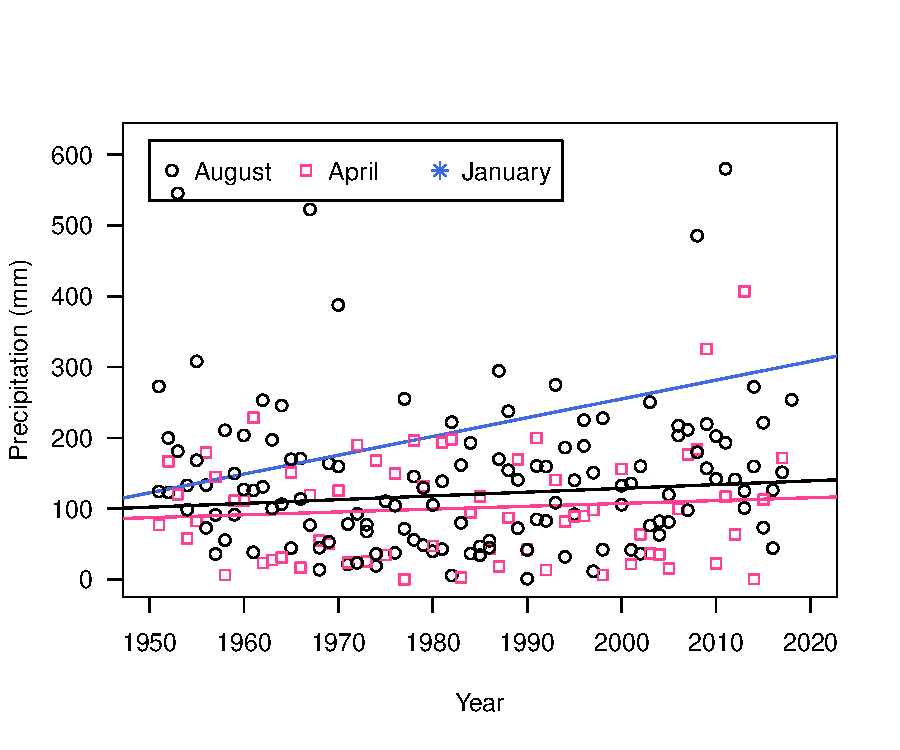
\includegraphics[width=.8\linewidth]{PRCP_Nakon}
%  \caption{?? in Nakon}
 % \label{fig:PRCP_Nakon}
%\end{figure}

%\textbf{Phuket}: Phuket's monthly average rainfall has been increasing from 1950 to the present day for the months of August, and January. August has a steep upward curve with a p value smaller than 0.05, the result is statistically significant. However, January, while an increasing curve, has a p value larger than 0.05, a statistically insignificant result. April's curve is decreasing, however, the p value is larger than 0.05, a statistically insignificant result. 

%\begin{figure}[h!]
%\centering
 % 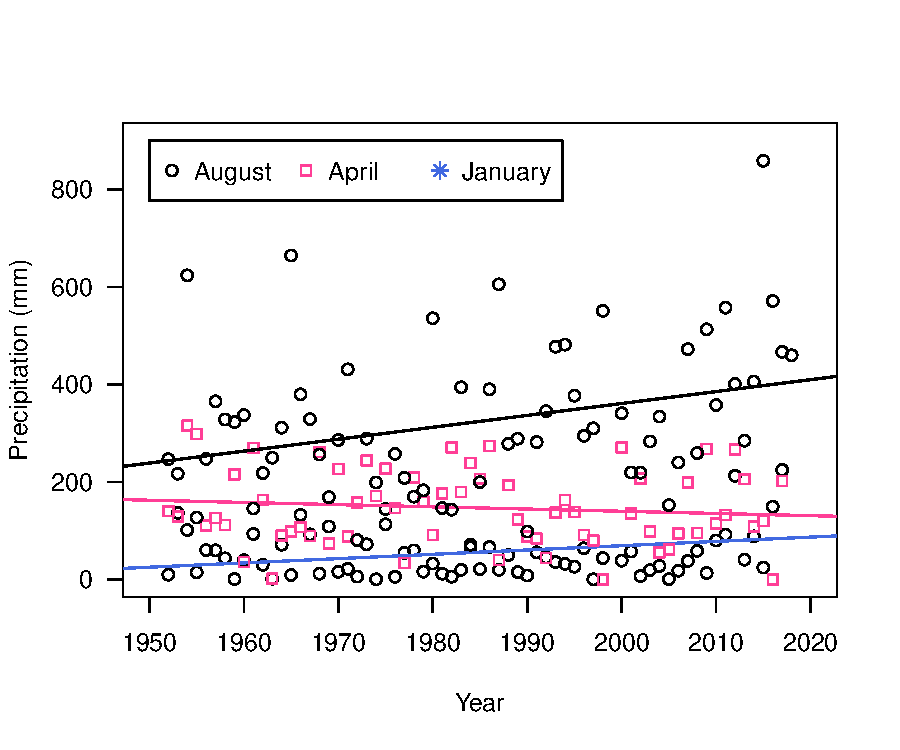
\includegraphics[width=.8\linewidth]{PRCP_Phuket}
%  \caption{Monthly Average Rainfall in Phuket}
 % \label{fig:PCRP_Phuket}
%\end{figure}

\subsubsection{Chapter exercise: temperature and rainfall graphs}
Now that you know what temperature and rainfall graphs look like, pick your own region and download data for it from NOAA $($https://www.ncdc.noaa.gov/cdo-web/$)$. Make your own temperature or rainfall graph! Does it agree with the temperature and rainfall trends of Bangkok and Singapore?

\subsection{Why are temperatures rising in Bangkok and Singapore?}

\subsubsection{Climate in South East Asia}

The climate of South East Asia itself might be contributing to climate patterns and variability. The weather in South East Asia is controlled by two dominant factors: the wet and the dry season (also called monsoon season). 
However, countries that are situated near the equator, such as Indonesia, Malaysia, southern Philippines, and Singapore have a tropical equatorial climate, and are consistently humid and wet throughout the year.  These countries do not experience variability in climate, and so they mostly do not experience typhoons, nor do they experience cool dry periods either. 

\subsubsection{Monsoons}

\subsubsection{What is a Monsoon?}
A Monsoon is the seasonal change in the direction and pressure of the prevailing winds that can lead to precipitation in a region. They are also the cause of wet and dry seasons in South East Asia. \citep{monsoonform}

\subsubsection{How do Monsoons form?}
Monsoons always blow from cold areas, where there is high pressure, to warm areas, where there is low pressure. The summer Monsoon and the winter Monsoon determine the climate for most of India and Southeast Asia. \citep{monsoonform}
 
\subsubsection{Summer Monsoon/Southwest Monsoon}
In Summer, between the months of April and September, the Asian landmass is warmer than the ocean, and so the density and the pressure of the air over the ocean is higher than the land. This causes a large amount of wet oceanic air to blow into inland Asia from the ocean, generating continuous precipitation and a humid climate. In the summer months, the Asian inland is heated up by the sun, causing temperatures to rise quickly. This creates an extensive low pressure region, leading the air to intensly flow from the Indian Ocean towards the land, leading to torrential rainfall in countries such as Vietnam, Thailand, and Myanmar. \citep{monsoonform}

\subsubsection{Winter Monsoon/North East Monsoon}
In winter, the Asian landmass is colder than the ocean, and so the density and the pressure of the air over the land is higher than the ocean. This causes a large amount of cold dry air to blow over the land until it reaches the ocean. Thus, the winter monsoon is called the dry season, as the air that is travelling across the land to the ocean does not receive any moisture until it reaches the ocean. When the cold front edge arrives at the sea area near Taiwan via the East China Sea, along with it comes the Northeast Monsoon with substantially strong winds. The Winter Monsoon normally lasts from October to April and starts to blow from the northeast. These winds start in the air above Mongolia and northwestern China. However, Winter Monsoons are less powerful than Summer Monsoons in Southeast Asia, in part because the Himalaya Mountains prevent much of the wind and moisture of the monsoons from reaching the coast. \citep{monsoonform}
 
 \begin{figure}[h!]
  \centering
  \includegraphics[width=\linewidth]{AsianMonsoon}
  \caption{The cycle of summer and winter moonsons in Asia. In the figure, the arrows represent moisture-laden winds.}
  \label{fig:asianmonsoon}
\end{figure}
 
\subsubsection{Impacts of Monsoons}
Billions of people around the globe depend on Monsoon rains for their yearly rainfall. For example, farmers in Myanmar�s Rakhine state need the rainfall from the Wet Monsoon season to cultivate paddy rice, especially since the Summer Monsoon brings in 80\% of the subcontinents rainfall. As agriculture contributes to 37.8\% of Myanmar�s economy, the arrival of the Monsoon season is crucial to the livelihoods of many citizens of Myanmar. \citep{monsoonimpact}

However, intense rainfall in these regions can cause massive flooding and mudslides, destruction of crops, and kill hundreds of people in floods. For example, during extreme Monsoon weather in Myanmar in 2015,  more than 1.4 million acres of farmland was flooded. Twelve out of the country's 14 provinces were affected, with northern and western regions suffering the hardest blows.385,000 households have been displaced by the floods, and landslides have destroyed thousands of homes. \citep{monsoonimpact}

\subsubsection{Monsoons in the future}
According to the IPCC, all models and all scenarios project an increase in both the mean and extreme precipitation in the Summer Monsoon. This could lead to major flooding events, especially in Southeast Asia.\citep{monsoonfuture}

\subsubsection{Effect of Monsoons on typhoons}
Typhoons normally occur during the same time as the Summer Monsoons, as they are strongest between the months of June through November in Southeast Asia. Wind pulls moisture from the warm oceans, and as the moisture floats upwards it is converted into warm air and heat. The heat causes more air to flow to the center of the storm, causing evaporation. Finally, all of the heat and air flow towards the eye, creating a typhoon. Due to warming seas, the destructive power of the typhoons that wreak havoc across Indonesia and the Philippines has intensified by 50\% in the past 40 years. Researchers warn that global warming will lead giant storms to become even stronger in the future, threatening the large and growing coastal populations of those nations. Typhoons can have devastating impacts in east Asia. In 2013, typhoon Haiyan hit the Philippines, killing at least 6,300 people and affecting 11 million \citep{typhoon}.

\subsubsection{Chapter Exercise: Monsoons}
Now that you know something about Monsoons, try drawing a diagram to demonstrate the difference between the Summer and the Winter Monsoon. Print out a map of South East Asia and add arrows to the map to show the different directions that te wind will move in!

\subsubsection{El Ni\~no-Southern Oscillation (ENSO) cycle}

The ENSO cycle is a scientific term that describes the fluctuations in temperature between the ocean and atmosphere in the east-central Equatorial Pacific area. The cycle is a natural phenomenon and includes El Ni\~no and La Nina, with both processes occurring from December to February \citep{enso}. 

\begin{figure}[h!]
  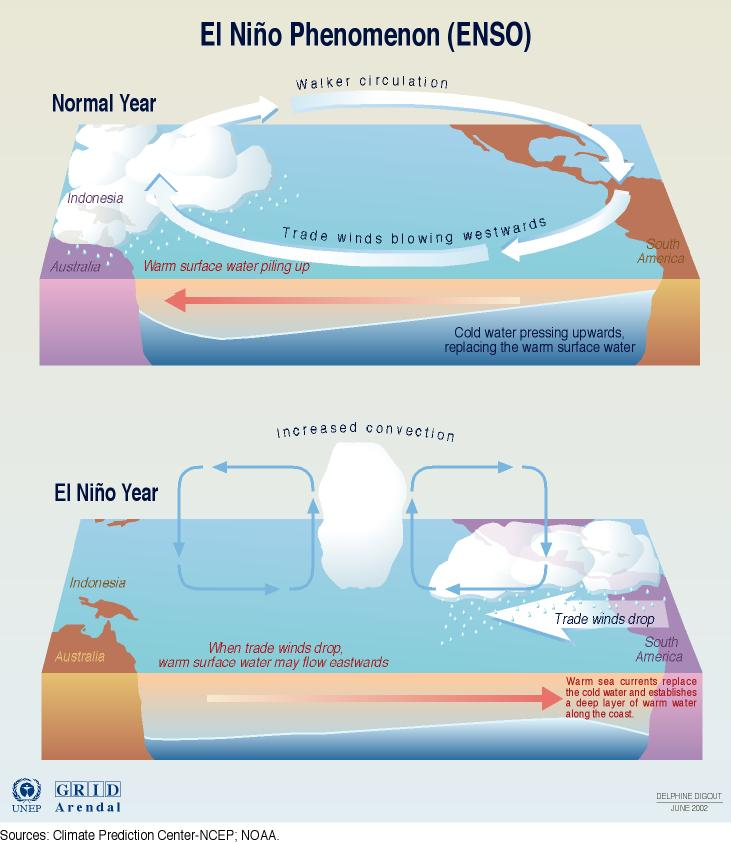
\includegraphics[width=\linewidth]{ENSO}
  \caption{The El Ni�o Cycle. Figure via the Climate Prediction Center of the NOAA National Centers for Environmental Prediction.}
  \label{fig:ENSO}
\end{figure}

\subsubsection{What is El Ni\~no}
El Ni\~no occurs every three to five years and begins when warm water in the western tropical Pacific Ocean shifts eastward along the equator toward the coast of South America. Normally, this warm water pools near Indonesia and the Philippines. However, during an El Ni\~no, the Pacific's warmest surface waters sit offshore of northwestern South America. This leads to Southeast Asia�s hot and dry climate, which usually occurs around the month of April, as the moisture is shifted towards South America \citep{enso}. 

\subsubsection{Effects of El Ni\~no}

One of the strongest El Ni\~no event in Southeast Asia happened in 1997. Then, fires, fueled by a drier rainy season in many parts of Indonesia, burned an estimated 5 million hectares, creating a haze that affected most of the region. The dry weather also caused massive food shortages in Indonesia, causing the government to import 5.8 million tons of rice due to drought and fire-related crop failures. Looking at the model predictions for the next 50 years, the researchers found that the impact of climate change could amplify the effects of each El Ni\~no, leading to temperature records being broken more often. However, researchers also mentioned that preparedness could allow societies in this region to cope with climate change. Since El Ni\~no can potentially be predicted a few months in advance, this could help societies prepare for extreme drought \citep{elninoindo}. 

\subsubsection{What is La Nina}
La Nina is the cooling of sea surface temperatures in the eastern and central Pacific. In general, this triggers wetter weather in South-East Asia and parts of Australia. Unusually strong, eastward-moving trade winds and ocean currents bring cold water to the surface east of the pacific ocean, a process known as upwelling. This leads to high air pressure in the east pacific, leading the air to flow to the western pacific, where the air pressure is lower and the temperatures are higher. These low-pressure zones contribute to increased rainfall in Southeast Asia \citep{enso}. 

\begin{figure}[h!]
  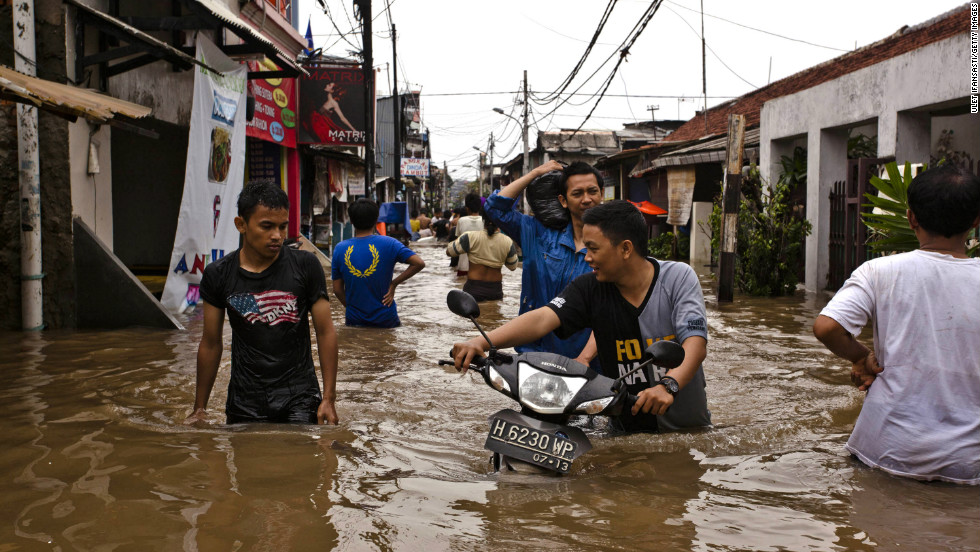
\includegraphics[width=\linewidth]{JakartaFloods}
  \caption{Flooding in Jakarta, Indonesia}
  \label{fig:jakartafloods}
\end{figure}

\subsubsection{Effects of La Nina}
Persistent heavy rains from La Nina led to flooding and landslides throughout Indonesia in late December 2007 and early January 2008, resulting in numerous fatalities and crop losses. The most heavily populated island in the chain, Java, was the hardest hit, and at least 112 people died on the island from flooding or landslides. \citep{elninoindo}.

\subsubsection{The Urban Heat Island Effect}
The Urban Heat effect occurs when heat and air temperature in densely built urban areas are higher than in the surrounding areas. This occurs when there is a lack of vegetation and soil moisture, which would normally be used to absorb the sunlight to evaporate water through photosynthesis. The heat that is absorbed during the day through buildings, roads, and other types of construction is reemitted during the night. The heat's energy contributes to raising the temperature of the surfaces and air around the urban areas. Furthermore, buildings can block wind, a cooling factor, which further leads to higher temperatures in cities. \citep{urbanheatisland}.  

Singapore has shown to be affected by the urban heat island effect, as shown in our graph by the steep increase in maximum temperature. According to a study published by the National University of Singapore, the high rise central district has a  2�C higher temperature at night compared to other areas with low-rise buildings. As the maximum temperature graph shows, maximum temperature in Singapore has been steeply increasing,  \citep{{singaporeclimatechange}}. 

Bangkok, the most developed and urban area in Thailand, is also affected by the urban heat island effect, as shown in our graph by the steep increase in maximum temperature. According to a study published by Istanbul University, Bangkok has  a 0.8�C higher temperature than the surrounding states of Bangkok \citep{bkkweather}. 

\subsubsection{Chapter Exercise: The Urban Heat Island Effect}
On a map, mark the cities, suburbs, rural areas and water bodies in the region where you live. Using the internet, find the average temperatures for these places in any given month and add this information to your map. Can you see the urban heat island in effect, as in Figure \ref{fig:urbanheat}?.

\begin{figure}[h!]
  \includegraphics[width=\linewidth]{UrbanHeatIslandEnhanced}
  \caption{The Urban Heat Island Effect}
  \label{fig:urbanheat}
\end{figure}

\subsection{Does the observed variability have anything to do with human forcing?}

In recent times, increasing awareness of the phenomenon of anthropogenic climate change has led to an increased effort to examine the role of human forcing in observed weather conditions and long-term climate trends. Greenhouse gas forcing has been tied to the patterns of anomalously high rainfall in the pre-Monsoon season leading up to the great flood of 2011 in Thailand, and thus these greenhouse gas emissions functioned as one of the forcing mechanisms for the flood itself \citep{floodfailure}. 

\section{What are the socio-economic implications for the countries analyzed?}

Our climate affects everything around us, including vital life indices. As long term climate change trends are being uncovered in meteorological data, a large number of studies are being published on the impact of these changes on essential factors such as food availability, the spread of diseases, water access and infrastructure. 

\subsection{Healthcare}
In Thailand, the occurence of liver fluke exhibits a strong positive correlation with precipitation and temperature, two factors which are being impacted by climate change \citep{liverfluke}. Temperatures in Thailand are clearly rising, as shown in Figure \ref{fig:TMAX_bangkok}, and the patterns of precipitation in the country are changing, as shown in Figure \ref{fig:PRCP_bangkok}. It is likely that liver fluke may exacerbated by ongoing climate changes.

In Singapore, the number of dengue cases was found to be correlated with temperature, but no statistically significant relationship was found with precipitation or humidity \citep{singaporedengue}. Temperatures in Singapore are also clearly rising, as shown in Figure \ref{fig:TMAX_Singapore} which means the number of dengue cases is forecasted to increase as well.

The comparision of Singapore to Thailand here can also be thought of in terms of their relative wealth. Singapore is situated in a region where vector-born diseases like dengue are endemic. However, because it is wealthy, the effects of climate change have not caused too many public health problems there. In fact, Singapore is the country which has made the most progress towards achieving health related UN Sustainability Goals \citep{sinagaporeclimatechange}. Thailand, on the other hand, is developing nation. It is much more prone to the occurence of a public health crisis through increased occurence of both insect-borne and water-borne diseases. In fact, the World Health Organization predicts that over 70 million people in Thailand will be at a signficant risk of contracting malaria \citep{borgen}.

\subsection{Water access}

Singapore is widely known as a country with a water scarcity problem. Climate change is expected to create significant sea level rise and temperature increase in Singapore by 2100, which will further stress the country's water resources, and have led it to establish a National Climate Chage Committee, which has enacted policies to protect the country from coastal erosion, flooding and loss of vital water supply \citep{bhullar2013climate}. 

Thailand does not have as much of a water scarcity problem, but significant degradation of forests and projected land use changes in the near future, combined with projected decreases in rainfall, are expected to decrease the yield and increase the sediment load of the Thadee watershed, a major source of water for agriculture and household use in the Nakhon Srithammarat Province in Southern Thailand \citep{landuse}. 

\begin{figure}
  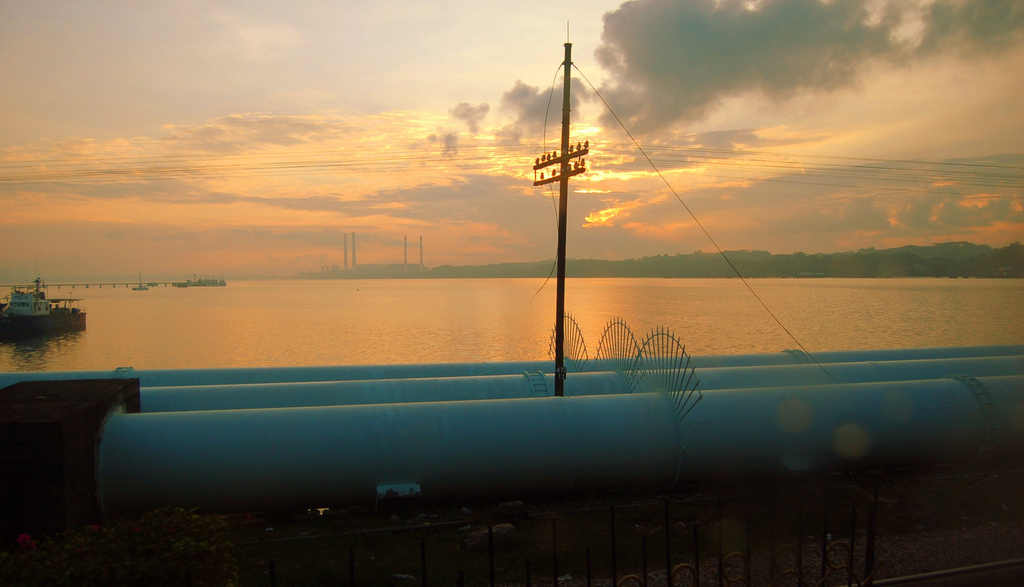
\includegraphics[width=\linewidth]{singaporepipe}
  \caption{The water pipeline at the Johor-Woodlands Causeway which brings 54\% of Singapore's water supply from Malaysia\citep{shaaz2008}}
  \label{fig:waterpipe}
\end{figure}

\subsection{Food}
An analysis of the climate indices that most affect rice production in Southeast Asia, specifically the onset of the wet season and nighttime temperatures, found that over the period from 1971-2012, nighttime temperatures were found to have increased, as shown in Tigure \ref{fig:TMAX_bangkok}, which has had an adverse effect on rice yields \citep{riceindices}. 

Poorer farmers are especially vulnerable to changing climate. An economic analysis of the impact of climate change on rice yields in Thailand which integrates soil science crop modeling, weather simulators, and global climate change modeling found that �overall, farmers are unable to neutralize the adverse effects of the more extreme climate change. However, they are able to cope with milder climate change and even benefit slightly from small increases in rainfall. While most farmers manage to adjust to milder climate change, poor farmers are less able to do so" \citep{climatechangerice}. Farmers' perceptions of changes in temperature and precipitation are generally consistent with the trends seen in Figures \ref{fig:TMAX_Singapore} and \ref{fig:PRCP_bangkok}. Agricultural experiences, farm income, training, social capital, and effective
climate adaptation communication are all significant factors in increasing the probability of them adapting to these climate changes \citep{farmerintention}.

The mountains of Northeast Thailand mostly see farming of low-value crops, which can be grown equally well in the lowlands. A study found that these mountains have a distinct advantage for the production of high-value fruits and vegetables, and planting of these high value crops represents a significant opportunity for agricultural development. citep{mountains}.  However, these fruits and vegetables are suited for temperate climates, and the potential for their cultivation may be impacted by the warming trend shown in figure \ref{fig:TMAX_bangkok}. 

Singapore, unlike Thailand, is not an agricultural hotspot. It imports over 90\% of its food , which makes it particularly vulnerable to fluctuations in global food supply and prices \citep{singaporeclimatechange}. 

\subsection{Biodiversity}

Changes in climatic conditions are having a massive impact on biodiversity all over the world. Because species evolve over long periods of time to live within certain range sof temperature, it is projected that by 2050,  25\% of all species will become extinct just because of rapid, anthropogenically induced climate change \citep{harvardbio}. 

Many species have responded to climate change by shifting their habitation ranges polewards, to avoid the warmer temperatures developing in pervading their original habitats. In Thailand, protected areas, which are on average 2�C cooler than the surrounding regions, are becoming increasingly vital for conservation of organisms such as tropical butterflies. Their importance is being further accentuated by the fact that most protected areas in Thailand are located at higher elevations, making them well suited to become habitats for species of butterflies migrating from lower elevations \citep{butterflies}. 

Biodiversity conservation measures in Southeast Asia may be impeded by a lack of willingness on the part of the local populations. For instance, a study conducted in households in China, Vietnam, the Philippines and Thailand found that people place a low priority on the conservation of animals such as marine turtles, and would be unwilling to accept additional taxes for conservation measures. This is likely a result of the fact that per-capita incomes in the region are generally not as high as in Western nations, and people do not trust government expenditure systems. This makes biodiversity conservation in the region something that may require international, rather than just local attention \citep{turtles}. 

For more on biodiversity and climate change, see \textbf{Chapter 6: Biomass}. 

\subsection{Air Quality}
Air quality is closely related to meteorological factors such wind speed, humidity, temperature, rainfall and solar radiation.  In Singapore, air quality standards have generally met the standards of the United States Environmental Protection Agency $($EPA$)$ and the World Health Organization $($WHO$)$ \citep{singaporeaq}. However, it is affected by the Southeast Asian Haze, which results from the slash and burn practices prevalent in the forests of Indonesia. This haze can make the air in Singapore dangerous to breathe. Understanding and combating this haze requires us to look into aerosol transport in the region using weather research and forecasting models \citep{singahaze}. The El Nino climate phenomenon described in \ref{fig:ENSO} can create exceptionally dry conditions in Indonesia, which can exacerbate forest fires there, and, by extension, the haze \citep{bbchaze}.   
For more on the Southeast Asian Haze, consider reading \textbf{Chapter 7: Peatlands}. 

\begin{figure}
  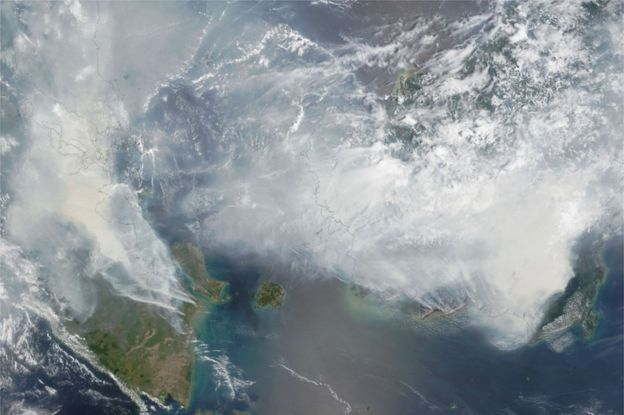
\includegraphics[width=\linewidth]{seasiahaze}
  \caption{A NASA satellite image of forest fires over Indonesia, which cause the Southeast Asian Haze \citep{bbchaze}}
  \label{fig:seaasiahaze}
\end{figure}

In Bangkok, a study has shown that there is a positive correlation between the trend of increasing temperatures seen in Figure \ref{fig:TMAX_bangkok} and PM2.5 concentrations. The city's air quality is already below the standards set by Thailand's Pollution Control Department, so climate change is exacerbating the problem. These increased PM2.5 concentrations are correlated with increased occurences of respiratory and circulatory diseases \citep{airpolchapter}. 

\subsection{Infrastructure}

The dual challenge of both mitigating and adapting to the effects of climate change are significant ones. Policymakers and scientists need to seek inspiration from a variety of sources to design effective solutions. Incorporation of local and indigenous knowledge into climate change mitigation strategies is essential for this purpose. 

For instance, small island communities in Indonesia, the Philippines and Timor Leste, which are particularly vulnerable to the effects of climate change such as sea level rise,  have extensive knowledge of climate mitigation strategies. These include the use of local materials for reinforcement of coastal structures, the use of alternative sources of food during hazards, and the use of knowledge of celestial bodies and the behavior of animals for local systems of weather forecasting. They even have traditional seasonal calendars \citep{indig}. The incorporation of the knowledge of these communities into more widespread systems of western-centric science could go a long way towards developing effective climate change mitigation and adaptation strategies for coastal communities thruoghout the region. 

Larger cities face their own set of climate-related infrastructure challenges, such as that of the urban heat island effect, which is likely to acerbated by climate change, and will require a variety of architectural and technological innovations to mitigate \citep{urbanheatisland}. Additionally, cities like Singapore and Hong Kong, which already require singificant electrical energy, may see an increase of between 3-5\% in the demand for electricity for every �C of temperature increase due to global warming \citep{singaporehongkong}. The problem of increased demand for energy can be extended to entire countries as well; a study of specific climate and ocioeconomic scenarios indicated that annual temperatures in Thailand will rise by 1.74 to 3.43 �C by 2080, implying increases in Thai peak electricity demand of 1.5-3.1 \% in the 2020s, 3.7-8.3\% in the 2050s, and 6.6-15.3\% in the 2080s \citep{thailandelectricity}. 

Slow coolant phaseout could worsen warming
April Reese
 See all authors and affiliations

Science  09 Mar 2018:
Vol. 359, Issue 6380, pp. 1084
DOI: 10.1126/science.359.6380.1084

For more on sea level rise, a significant infrastructural challenge that results from climate change, see \textbf{Chapter 9: Sea Level Rise and Subsidence}. 

\section{The Policy Context}
\subsubsection{ASEAN}
Singapore and Thailand are both part of the Association of Southeast Asian Nations $($ASEAN$)$, as well as other international iniatives such as the Intergovernmental Panel on Climate Change $($IPCC$)$. ASEAN, in particular, enables cooperation on responses to climate change in a South East Asian context \citep{asean2015}. For instance, businesses in some ASEAN countries have incorporated greenhouse gas emission reductions and fuel efficiency into their operations as they are aware of climate change and its potential impacts on ASEAN countries, which have fragile natural environments \citep{aseanbusiness}. However, ASEAN members so far have done little to curtail instances of cross-border pollution, and there are other limitations inherent in the organization's climate policy. 

Individual states within ASEAN have often done better than the organization as a whole. For instance, Malaysia has a long-run carbon emissions policy which is superior to that of ASEAN as a whole. It will, in the long run, enhance Malaysia's economy through the stimulation of the green technology sector, and the mitigation of the future costs of climate change related damage \citep{aseanmalaysia}. 

Pan-ASEAN policies have been effective in some areas, however. For instance, its member
countries signed the ASEAN Agreement on Transboundary Haze Pollution in 2012 in
order to prevent, monitor, and mitigate fires. This was done in order to combat the the transboundary haze pollution described before. Even Indonesia, the source of most of the fires, signed the agreement in 2014. A related measure, the ASEAN Peatland Management Initiative $($APMI$)$, has also been implemented over the period from 2006-2020. The APMI was  developed to guide ASEAN countries to sustainably manage peatlands and reduce fires and associated haze within the framework of the ASEAN Agreement on Transboundary Haze Pollution. Under the ASEAN umbrella, Singapore has been able to explore sanctioning Indonesia in order to get it to crack down on the agricultural practices responsible for the Southeast Asian Haze \citep{singahongkong}.  

\subsection{Change at the community level}
In regions that are especially vulnerable to climate change effects, adaptation is already taking place at the community and household level. There is an established history of grassroots movements in Southeast Asia, and this can enable the linking of both autonomous and planned adaptation planning to disaster risk management planning. National governments and international agencies can achieve good results just by supporting such grassroots level efforts. Funding under initatives such as the United Nations Framework Convention on Climate Change $($UNFCC$)$ and the Kyoto Protocol is crucial \citep{adaptationseasia}

\subsection{International Perspective}
All Southeast Asian nations are party to the Paris Climate Agreement signed in 2015. Given the significant challenges faced by countries in the region due to sea level rise, transboundary haze, extreme weather events and food insecurity, the Global Climate Risk Index states that four of the top ten countries most vulnerable to climate change are in this region; Thailand, Vietnam, Myanmar and the Philippines \citep{WRIasean}. The standards set in the Paris Agreement, if met, will help these nations with some of their problems. However, even if global warming is kept below 2�C over pre-industrial levels by 2100, Southeast Asia may still see a sea-level rise of about 75 centimeters, which would be catastrophic. The countries in the region may well have to go above and beyond the standards set in the Paris Agreement. The agreement will be helpful in that developed countries that signed it have pledged to support developing countries in their climate change adaption to the tune of USD 100 billion (92.3 billion euro) annually from 2020 on. This financial support will likely go a long way towards helping developing Southeast Asian nations curtail carbon emissions and develop clean technologies \citep{DW2015}. 

\section{Conclusion}
For better or worse, our existence on this planet has caused significant changes to the planet's vital systems. The planet is now continously responding and evolving in response to our actions. Sometimes, these responses can be destructive. Meteorology, and the closely related field of climatology, are crucial because they help us determine future weather and climate expectations. In a world where climate is changing rapidly, it is crucial for us to effectively observe and model climatological variables, so we can stay ahead of the curve. This is especially important in East and Southeast Asia, where climate change is driving changes in socio-economic sectors vital to our lives, such as healthcare, food, water access and agriculture. 
Going forward, we need to continue to expand our capacity to observe and predict our weather and climate. This is so that we can stop more natural disasters before they happen, predict climatic changes that will affect vital life sectors and industries, and, perhaps most importantly, continously remind ourselves of the need to adopt sustainability measures. It is fair to say that while climatological and meteorological data is essential in helping us survive today, it is even more essential in helping us plan for tomorrow. 

